\documentclass[11pt,letterpaper]{article}
\usepackage[top=3cm, bottom=2cm, left=2cm, right=2cm, columnsep=20pt]{geometry}
\usepackage{pdfpages}
\usepackage{graphicx}
\usepackage{etoolbox}
\apptocmd{\sloppy}{\hbadness 10000\relax}{}{}
% \usepackage[numbers]{natbib}
\usepackage[T1]{fontenc}
\usepackage{ragged2e}
\usepackage[french]{babel}
\usepackage{listings}
\usepackage{color}
\usepackage{soul}
\usepackage[utf8]{inputenc}
\usepackage[export]{adjustbox}
\usepackage{caption}
\usepackage{amsmath}
\usepackage{amssymb}
\usepackage{float}
\usepackage{csquotes}
\usepackage{fancyhdr}
\usepackage{wallpaper}
\usepackage{siunitx}
\usepackage[indent]{parskip}
\usepackage{textcomp}
\usepackage{gensymb}
\usepackage{multirow}
\usepackage[hidelinks]{hyperref}
\usepackage{abstract}


\renewcommand{\abstractnamefont}{\normalfont\bfseries}
\renewcommand{\abstracttextfont}{\normalfont\itshape}
\usepackage{titlesec}
\titleformat{\section}{\large\bfseries}{\thesection}{1em}{}
\titleformat{\subsection}{\normalsize\bfseries}{\thesubsection}{1em}{}
\titleformat{\subsubsection}{\normalsize\bfseries}{\thesubsubsection}{1em}{}

\usepackage{xcolor}
\definecolor{codegreen}{rgb}{0,0.6,0}
\definecolor{codegray}{rgb}{0.5,0.5,0.5}
\definecolor{codepurple}{rgb}{0.58,0,0.82}
\definecolor{backcolour}{rgb}{0.95,0.95,0.92}
\lstdefinestyle{mystyle}{
    backgroundcolor=\color{backcolour},   
    commentstyle=\color{codegreen},
    keywordstyle=\color{magenta},
    numberstyle=\tiny\color{codegray},
    stringstyle=\color{codepurple},
    basicstyle=\ttfamily\footnotesize,
    breakatwhitespace=false,         
    breaklines=true,                 
    captionpos=b,                    
    keepspaces=true,                 
    numbers=left,                    
    numbersep=5pt,                  
    showspaces=false,                
    showstringspaces=false,
    showtabs=false,                  
    tabsize=2
}
\lstset{style=mystyle}

\usepackage[most]{tcolorbox}
\newtcolorbox{note}[1][]{
  enhanced jigsaw,
  borderline west={2pt}{0pt}{black},
  sharp corners,
  boxrule=0pt, 
  fonttitle={\large\bfseries},
  coltitle={black},
  title={Note:\ },
  attach title to upper,
  #1
}

%----------------------------------------------------

\setlength{\parindent}{0pt}
\DeclareCaptionLabelFormat{mycaptionlabel}{#1 #2}
\captionsetup[figure]{labelsep=colon}
\captionsetup{labelformat=mycaptionlabel}
\captionsetup[figure]{name={Figure }}
\newcommand{\inlinecode}{\normalfont\texttt}
\usepackage{enumitem}
\setlist[itemize]{label=\textbullet}

\begin{document}
\begin{titlepage}
\center

\begin{figure}
    \ThisULCornerWallPaper{.4}{Polytechnique_signature-RGB-gauche_FR.png}
\end{figure}
\vspace*{2 cm}

\textsc{\Large \textbf{PHS3910 --} Techniques expérimentales et instrumentation}\\[0.5cm]
\large{\textbf{Équipe : Lundi 03}}\\[1.5cm]

\rule{\linewidth}{0.5mm} \\[0.5cm]
\Large{\textbf{Microscope pour suivi de particules}} \\[0.2cm]
\text{Fiche technique}\\
\rule{\linewidth}{0.5mm} \\[2.3cm]

\large{\textbf{Présenté à}\\
  Jean Provost\\
  Lucien Weiss\\[2.5cm]
  \textbf{Par :}\\
  Émile \textbf{Guertin-Picard} (2208363)\\
  Philippine \textbf{Beaubois} (2211153)\\
  Marie-Lou \textbf{Dessureault} (2211129)\\
  Maxime \textbf{Rouillon} (2213291)\\[3cm]}

\large{\today\\
Département de Génie Physique\\
Polytechnique Montréal\\}

\end{titlepage}

%----------------------------------------------------

\tableofcontents
\pagenumbering{roman}
\newpage

\pagestyle{fancy}
\setlength{\headheight}{14pt}
\renewcommand{\headrulewidth}{0pt}
\fancyfoot[R]{\thepage}

\pagestyle{fancy}
\fancyhf{}
\renewcommand{\headrulewidth}{1pt}
\fancyhead[L]{\textbf{PHS3910}}
\fancyhead[C]{Fiche technique du microscope}
\fancyhead[R]{\today}
\fancyfoot[R]{\thepage}

\pagenumbering{arabic}
\setcounter{page}{1}

%----------------------------------------------------

\section{Description générale et spécifications}

Cette fiche technique, à la demande du Gouvernement du Québec, présente les caractéristiques 
d'un microscope servant au suivi de microparticules contaminants l'environnement près de 
l'usine Polyfab \textcolor{red}{lol}. Les composantes principales sont un laser 405 nm (CPS405)
pour illuminer les fluorophores dans les échantillons, un objectif de microscope (grossissement 
$M = 20$, aperture NA $= 0.4$) pour le grossissement, puis une lentille tube de 150 mm de focale
(LA1433-A-ML) pour converger les rayons sortants de l'objectif sur le capteur d'une caméra CMOS 
(CS165MU) pour l'analyse \textcolor{red}{Source Thorlabs}. Ce système présente une résolution
théorique de 1.012 µm. Afin d'analyser des particules d'environ cette taille, un traitement
numérique est fait pour extraire la taille des particules du mouvement brownien filmé, avec 
une résolution sous-pixellaire. Avec ce procédé, le microscope peut détecter des tailles de 
particules dans la plage  \textcolor{red}{XX - XX} µm. Suite à la caractérisation de particules 
de 1 µm, l'erreur sur la valeur identifiée est de \textcolor{red}{XX $\pm$ XX} µm.
Pour la caractérisation de particules de 10 µm, l'erreur sur la valeur identifiée est de 
\textcolor{red}{XX $\pm$ XX} µm. Le système, monté sur table optique et utilisable dans le noir 
seulement, a des dimensions de \textcolor{red}{$600 \times 90 \times 200$} mm, tel que présenté à 
la figure \ref{schema_micro}. Sans compter la table, il a pour coût total 1483.59 \$, prix qui
peut être réduit par l'usage d'impression 3D.

% Source Thorlabs : https://www.thorlabs.com

\begin{figure}[H]
  \centering
  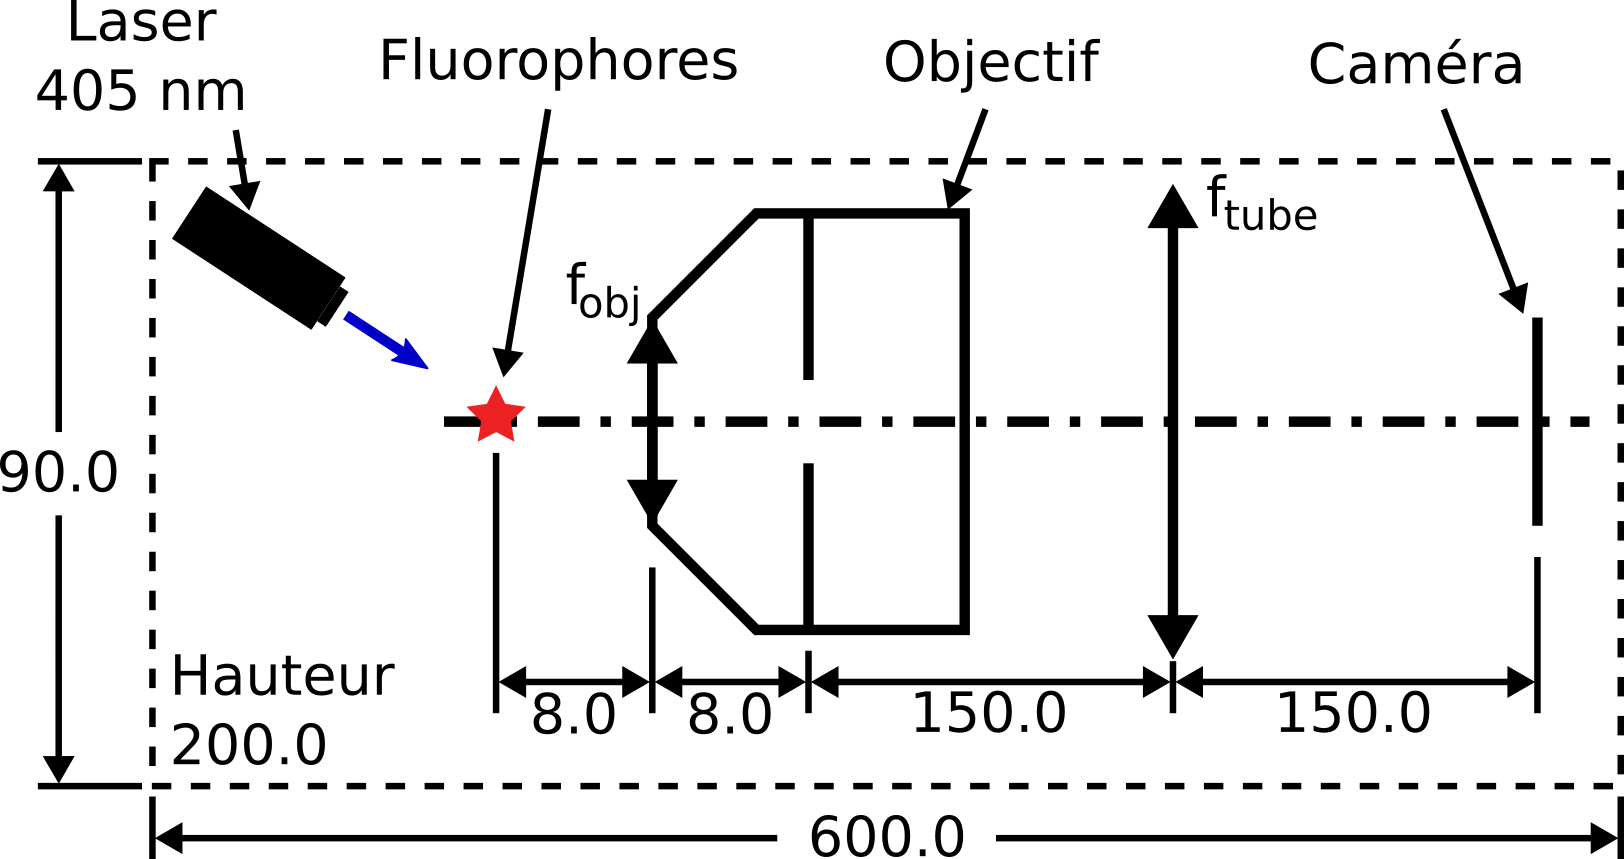
\includegraphics[scale=2.8]{schema_fiche_tech.png}
  \caption{Schéma du microscope avec les dimensions critiques. Toutes les dimensions sont en millimètres avec une tolérance de $\pm$ 1 mm.}
  \label{schema_micro}
\end{figure}



\section{Rapports de tests}

\subsection{Résolution sans analyse numérique}

\textcolor{red}{ce qui était dans le rapport préliminaire}


\subsection{Caractérisation de la taille de particules}
Lors de l'acquisition des images, il a été conclu que le temps d'exposition devait être assez long, environ 150ms. Par conséquent, pour espérer 
obtenir des images, il fallait réduire le temps d'acquisition, soit environ 2 images par seconde. Margé ces ajustements, la caméra ne parvient tout de même
pas a enregistré chaque image demandée et remplace les images non enregistrées par une image noire (environ 4 images noir pour 75 images au totales). Pour palier à cette contrainte et que celle-ci n'influence pas les divers calculs d'analyse,
 la procédure suivante a été choisie: 
Pour traité les images et pouvoir tracker les particules, toutes les images noir sont ignorées pour ne garder que les images analysables.
Une fois que la liste de position pour chaque image a été produite, toutes les images de départ sont toutes revues une par une, et à chaque fois qu'une
image noire apparaît un vecteur de $\left [ NaN ,NaN \right ]$ est ajouté au vecteur contenant toutes les positions.
 Cette procédure nous permet de savoir avec exactitude les emplacements des images qui n'ont pas pu être enregistrés. Une fois le vecteur de positions 
 complet, il est possible de de commencer le calcul de MDS avec la formule suivante: 
 \begin{align}
  MSD &= \frac{1}{N_{\Delta t}} \sum_{i=0}^{N_{\Delta t} - 1} \left( \mathbf{r}(i+\Delta t) - \mathbf{r}(i) \right)^2,\\ 
  \mathbf{r}(i) &= x(i)\hat{x}+ y(i)\hat{y}
\end{align}
L'incertitude sur ces valeurs sont donnée par les formule suivante: 
\begin{equation}
  \alpha =A+B
\end{equation}
\begin{align*}
  A = \sqrt{
    \begin{aligned}
      &\left( 2(x(i+\Delta t) - x(i))\cdot \Delta x(i+\Delta t) \right)^2 \\
      &+ \left( 2(x(i+\Delta t) - x(i))\cdot \Delta x(i) \right)^2
    \end{aligned}
  }
\end{align*}
\begin{align*}
  B = \sqrt{
    \begin{aligned}
      &\left( 2(y(i+\Delta t) - y(i))\cdot \Delta y(i+\Delta t) \right)^2 \\
      &+ \left( 2(y(i+\Delta t) - y(i))\cdot \Delta y(i) \right)^2
    \end{aligned}
  }
\end{align*}
\textcolor{red}{SOURCE: travail prep}

On remarque que c'est ici que le traitement de toutes les images est important, car sinon le $\Delta t$ n'aurait pas été cohérent avec la procédure de la MDS. 
La façon de traiter ce calcul avec les vecteurs $\left [ NaN ,NaN \right ]$ tout en perdant le moins d'information possible a été de définir que 
dès que l’élément NaN est détecté dans un calcul, $\left( \mathbf{r}(i+\Delta t) - \mathbf{r}(i) \right)=0$. De cette façon les images non enregistrées
ne peuvent pas interférer dans le calcul de la MDS. Dans la même idée, les incertitudes sur les positions étaient calculées à l'aide de l'écart-type 
du fit gaussien, dans le cas d'une image noire, on pose dx=0 et dy=0. Les images noir ne sont donc pas pris en compte non plus dans les calcul d'incertitude.  

Une fois toutes les valeurs trouvées, un graphique des résultat de MDS en fonction du $\Delta t$ est produit. 
Un fit quadratique est en suite effectuer sur les 5 premiers points de ce graphique, il est ainsi possible d'identifier les 3 coefficients de celle-ci.
Les incertitudes sur ces 3 valeurs sont données par la racine carrée de la diagonalisation de la matrice de covariance donnée par la fonction curve\_fit. 
C'est le coefficient B du fit qui sera utilisé pour trouver le coefficient de diffusion (D) et la taille de la particule (r). Les formules suivantes sont utilisées: 
\begin{align*}
  D &= \frac{B}{4} \quad & r &= \frac{k_B T}{6 \pi \eta D}
\end{align*}
L'incertitude sur chacune de ces valeurs est donnée par l'incertitude sur le coefficient B, car on considère que les autres paramètres sont des constantes
et ne comportent donc pas d'incertitudes. 

\textcolor{red}{Acquisition de données (paramètres d'acquisition, traitement des lost frames)}

\textcolor{red}{Tableau des résultats}

\subsubsection{Paramètres utilisés}



\subsection{Étude des coûts}

Une étude des coûts a été faite pour le microscope construit afin de voir s'il y a possibilité
de construire un appareil aux performances similaires, mais à moindre coût. Le tableau \ref{table_cout}
présente la liste exhaustive des pièces avec leur prix en dollars canadien avant taxes.

\begin{table}[!ht]
    \centering
    \caption{Liste des pièces et coûts totaux pour le microscope sur table optique
    \textcolor{red}{Source Thorlabs}.}
    \begin{tabular}{|l|l|l|l|l|}
    \hline
        ID pièce & Description & Qté & \$ CAD & Total ind. \\ \hline\hline
        KM100S & Montage ajustable pour échantillon & 1 & \$130.45 & \$130.45 \\ \hline
        CS165MU & Caméra CMOS monochrome & 1 & \$667.01 & \$667.01 \\ \hline
        - & Objectif de microscope & 1 & \$10.00 & \$10.00 \\ \hline
        420FDL12 & Filtre passe-long & 1 & \$36.29 & \$36.29 \\ \hline
        LA1433-A-ML & Lentille tube f = 150.0 mm & 1 & \$71.42 & \$71.42 \\ \hline
        CPS405 & Laser bleu 405 nm & 1 & \$312.07 & \$312.07 \\ \hline
        LMR1 & Trou taraudé pour lentilles & 2 & \$22.89 & \$45.79 \\ \hline
        TR3-P5 & 5 tiges 3 po pour optiques & 1 & \$38.50 & \$38.50 \\ \hline
        PH4 & Base pour tiges d'optique 4 po & 4 & \$14.83 & \$59.33 \\ \hline
        PH3 & Base pour tiges d'optique 3 po & 1 & \$13.37 & \$13.37 \\ \hline
        BA1 & Pied de montage optique & 1 & \$8.42 & \$8.42 \\ \hline
        BA1S & Pied de montage optique & 2 & \$7.83 & \$15.65 \\ \hline
        BA2 & Pied de montage optique & 1 & \$11.26 & \$11.26 \\ \hline
        VC1 & Pince en V & 1 & \$64.04 & \$64.04 \\ \hline\hline
        ~ & ~ & ~ & Total : & \$1483.59 \\ \hline
    \end{tabular}
    \label{table_cout}
\end{table}

% Source Thorlabs : https://www.thorlabs.com

Quelques éléments sont à souligner. Premièrement, étant donné que l'objectif de microscope a
été fourni par le gouvernement du Québec, le coût qui y est associé a été estimé selon leurs
informations. Ces objectifs sont de seconde main, et ils ont été achetés en ensemble. Cela mène
au faible coût d'environ 10\$, qui pourrait être difficile à retrouver pour la construction d'un
seul microscope. Toutefois, pour la construction d'un ensemble d'appareils spécialisés pour
différentes tailles de particules, donc ayant besoin de différents objectifs à différents 
grossissements, le prix d'ensemble est idéal. Deuxièmement, un coût important a été omis dans 
le tableau de calcul, soit celui de la table optique elle-même. Cette dernière est très
dispendieuse, mais elle a été omise car elle est déja présente dans plusieurs laboratoires 
d'optique, ou si non, elle peut être acheté à plus faible coût si les dimensions de la table
achetée se limitent aux dimensions de l'appareil. Par exemple, chez Thorlabs, la plus petite 
table optique pour tenir ce microscope est la B1824F, avec des dimensions de 18" $\times$ 24".
Avec un coût de 1319.08 \$ CAD, presque l'entièreté du coût du reste de l'appareil, le total
monte à 2802.67 \$. Troisièmement, selon le tableau \ref{table_cout}, les pièces ayant les
coûts les plus considérables sont celles directement lié à l'optique et à l'alignement. Le
reste des pièces sont pour des éléments de construction du montage, et leur total s'élève à
733.31 \$.

Il est donc possible de recommander fortement l'utilisation de l'impression 3D pour une production
à plus grand volume de ce microscope. Cela permettrat de sauver l'argent sur les pièces de
construction et sur la table optique elle-même, aiderait à l'alignement des éléments optiques,
permettrait plus de flexibilité sur les composantes à ajuster tel que le motage de l'échantillon pour
s'occuper du focus, et enfin pourrait rendre l'appareil plus portatif pour des essais sur le terrain.
Comme les éléments optiques seraient tous réutilisables dans un design d'impression 3D, les
performances du dispositif resteraient identiques. Il est aussi possible de recommander l'usage
d'un différent laser de 405 nm, car ils sont fréquemment vendus seconde main pour beaucoup moins
cher.

% \bibliographystyle{unsrtnat}
% \bibliography{My_Library}

\end{document}
